% Native TikZ overview. No extra TikZ libraries or external image files.
% Scope: uncapped exact-total simplex; noiseless internal prefix readings.
\begin{figure}[htbp]
\centering
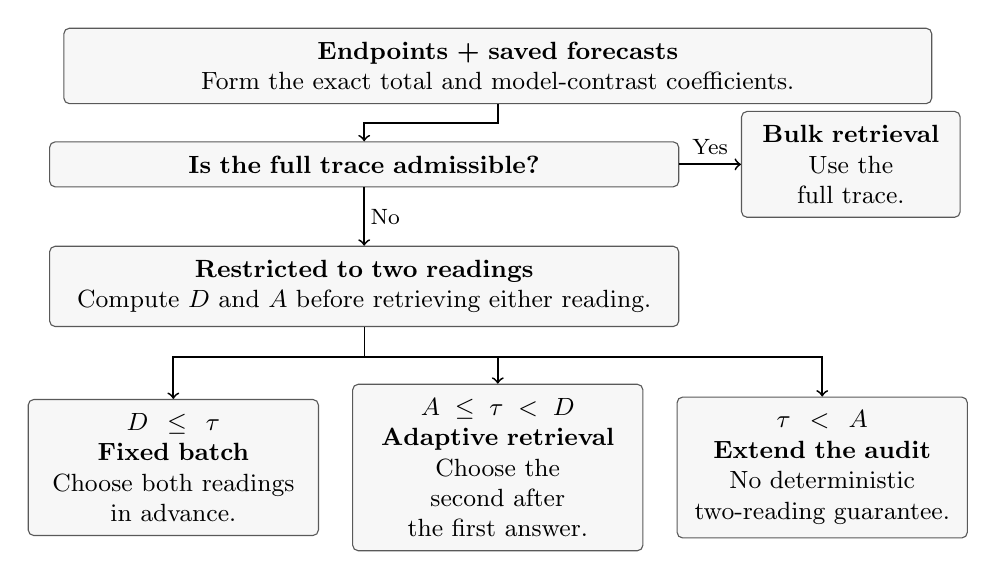
\begin{tikzpicture}[x=0.01\linewidth,y=1cm,
  every node/.style={font=\small,align=center},
  flowbox/.style={draw=black!65,rounded corners=2pt,fill=black!3,
    inner sep=5pt},
  flowarrow/.style={->,line width=0.65pt}]
\node[flowbox,text width=0.88\linewidth] (inputs) at (50,0)
  {\mbox{\textbf{Endpoints + saved forecasts}}\\
   Form the exact total and model-contrast coefficients.};
\node[flowbox,text width=0.63\linewidth] (access) at (36,-1.25)
  {\mbox{\textbf{Is the full trace admissible?}}};
\node[flowbox,text width=0.20\linewidth] (bulk) at (87,-1.25)
  {\mbox{\textbf{Bulk retrieval}}\\Use the full trace.};
\node[flowbox,text width=0.63\linewidth] (plan) at (36,-2.80)
  {\mbox{\textbf{Restricted to two readings}}\\
   Compute $D$ and $A$ before retrieving either reading.};
\node[flowbox,text width=0.275\linewidth] (fixed) at (16,-5.10)
  {$D\leq\tau$\\\mbox{\textbf{Fixed batch}}\\
   Choose both readings\\in advance.};
\node[flowbox,text width=0.275\linewidth] (adaptive) at (50,-5.10)
  {$A\leq\tau<D$\\\mbox{\textbf{Adaptive retrieval}}\\
   Choose the second after\\the first answer.};
\node[flowbox,text width=0.275\linewidth] (escalate) at (84,-5.10)
  {$\tau<A$\\\mbox{\textbf{Extend the audit}}\\
   No deterministic\\two-reading guarantee.};
\draw[flowarrow] (inputs.south) -- (50,-0.72) -- (36,-0.72)
  -- (access.north);
\draw[flowarrow] (access.east) -- node[above,font=\footnotesize]{Yes}
  (bulk.west);
\draw[flowarrow] (access.south) -- node[midway,right,inner sep=2pt,font=\footnotesize]{No}
  (plan.north);
\draw (plan.south) -- (36,-3.70) -- (50,-3.70);
\draw[flowarrow] (50,-3.70) -- (16,-3.70) -- (fixed.north);
\draw[flowarrow] (50,-3.70) -- (adaptive.north);
\draw[flowarrow] (50,-3.70) -- (84,-3.70) -- (escalate.north);
\end{tikzpicture}
\caption{Choosing an audit protocol. For the exact-total, noiseless prefix
model, let $J_Q=\max_r W_{r,Q}/W_{r,0}$ over contrasts with positive initial
width. Let $D=\min_Q\sup_y J_Q(y)$ and
$A=\min_{P\,\mathrm{det.\ adaptive}}\sup_y J_{Q_P(y)}(y)$ under the same
two-reading budget. We fix the target $\tau$ before retrieval; the main
application uses $\tau=1/2$. Since $A\leq D$, the three restricted-access
branches exhaust deterministic guarantee possibilities. Randomized precision
success is assessed separately. Bulk is preferred on the measured public
API when its full response is admissible (Section~\ref{sec:actual-api}).}
\label{fig:audit-workflow}
\end{figure}
